\documentclass[11pt]{aghdpl}
% \documentclass[en,11pt]{aghdpl}  % praca w języku angielskim

% Lista wszystkich języków stanowiących języki pozycji bibliograficznych użytych w pracy.
% (Zgodnie z zasadami tworzenia bibliografii każda pozycja powinna zostać utworzona zgodnie z zasadami języka, w którym dana publikacja została napisana.)
\usepackage[english,polish]{babel}

% Użyj polskiego łamania wyrazów (zamiast domyślnego angielskiego).
\usepackage{polski}

\usepackage[utf8]{inputenc}

% dodatkowe pakiety

\usepackage{mathtools}
\usepackage{amsfonts}
\usepackage{amsmath}
\usepackage{amsthm}

% --- < bibliografia > ---

\usepackage[
style=numeric,
sorting=none,
%
% Zastosuj styl wpisu bibliograficznego właściwy językowi publikacji.
language=autobib,
autolang=other,
% Zapisuj datę dostępu do strony WWW w formacie RRRR-MM-DD.
urldate=iso8601,
% Nie dodawaj numerów stron, na których występuje cytowanie.
backref=false,
% Podawaj ISBN.
isbn=true,
% Nie podawaj URL-i, o ile nie jest to konieczne.
url=false,
%
% Ustawienia związane z polskimi normami dla bibliografii.
maxbibnames=3,
backend=biber,
]{biblatex}

\usepackage{csquotes}
% Ponieważ `csquotes` nie posiada polskiego stylu, można skorzystać z mocno zbliżonego stylu chorwackiego.
\DeclareQuoteAlias{croatian}{polish}

\addbibresource{bibliografia.bib}

% Nie wyświetlaj wybranych pól.
%\AtEveryBibitem{\clearfield{note}}


% ------------------------
% --- < listingi > ---

% Użyj czcionki kroju Courier.
\usepackage{courier}

\usepackage{listings}
\lstloadlanguages{TeX}

\lstset{
	literate={ą}{{\k{a}}}1
           {ć}{{\'c}}1
           {ę}{{\k{e}}}1
           {ó}{{\'o}}1
           {ń}{{\'n}}1
           {ł}{{\l{}}}1
           {ś}{{\'s}}1
           {ź}{{\'z}}1
           {ż}{{\.z}}1
           {Ą}{{\k{A}}}1
           {Ć}{{\'C}}1
           {Ę}{{\k{E}}}1
           {Ó}{{\'O}}1
           {Ń}{{\'N}}1
           {Ł}{{\L{}}}1
           {Ś}{{\'S}}1
           {Ź}{{\'Z}}1
           {Ż}{{\.Z}}1,
	basicstyle=\footnotesize\ttfamily,
}

% ------------------------

\AtBeginDocument{
	\renewcommand{\tablename}{Tabela}
	\renewcommand{\figurename}{Rys.}
}

% ------------------------
% --- < tabele > ---

\usepackage{array}
\usepackage{tabularx}
\usepackage{multirow}
\usepackage{booktabs}
\usepackage{makecell}
\usepackage[flushleft]{threeparttable}
\usepackage[hidelinks, colorlinks=false]{hyperref}
\usepackage{longtable}

% defines the X column to use m (\parbox[c]) instead of p (`parbox[t]`)
\newcolumntype{C}[1]{>{\hsize=#1\hsize\centering\arraybackslash}X}

% lepsze pozycjonowanie figur
\usepackage{float}

% dla np. \degree jako symbol stopnia
\usepackage{gensymb}

% listingi kodu
\usepackage{listings}

%---------------------------------------------------------------------------

\author{Piotr Banaszkiewicz}
\shortauthor{P. Banaszkiewicz}

\titlePL{Wyłącznik awaryjny pojazdu autonomicznego}
\titleEN{Emergency Stop Autonomous Vehicle}


\shorttitlePL{Wyłącznik awaryjny pojazdu autonomicznego} % skrócona wersja tytułu jeśli jest bardzo długi
\shorttitleEN{Emergency Stop Autonomous Vehicle}

\thesistype{Praca dyplomowa inżynierska}

\supervisor{dr inż. Marek Długosz}

\degreeprogramme{Automatyka i Robotyka}

\date{2016}

\department{Katedra Automatyki i Inżynierii Biomedycznej}

\faculty{Wydział Elektrotechniki, Automatyki,\protect\\[-1mm] Informatyki i Inżynierii Biomedycznej}
%\faculty{Faculty of Electrical Engineering, Automatics, Computer Science and Biomedical Engineering}

\acknowledgements{Serdecznie dziękuję opiekunowi pracy, Panu Doktorowi Markowi Długoszowi, a także opiekunowi pracowni inżynierskiej, Panu Doktorowi Januszowi Tenecie, za niesioną pomoc i zawsze dobrą radę.}


\setlength{\cftsecnumwidth}{10mm}

%---------------------------------------------------------------------------
\setcounter{secnumdepth}{4}

\begin{document}

\titlepages

% Ponowne zdefiniowanie stylu `plain`, aby usunąć numer strony z pierwszej strony spisu treści i poszczególnych rozdziałów.
\fancypagestyle{plain}
{
	% Usuń nagłówek i stopkę
	\fancyhf{}
	% Usuń linie.
	\renewcommand{\headrulewidth}{0pt}
	\renewcommand{\footrulewidth}{0pt}
}

\setcounter{tocdepth}{2}
\tableofcontents
\clearpage

\chapter{Wstęp}
\label{cha:wstep}

Laboratorium pojazdów autonomicznych AGH—Delphi ma za zadanie zbudowanie pojazdu autonomicznego na bazie udostępnionego pojazdu elektrycznego (zob. zdjęcie \ref{fig:electric_vehicle}). Podczas prac konieczne jest zapewnienie bezpieczeństwa podczas testowania algorytmów sterowania. Algorytmy takie mogą nie działać poprawnie, w~związku z~czym w~trakcie testów może zajść potrzeba awaryjnego przerwania jazdy samochodu.

\begin{figure}[h]
	\centering
	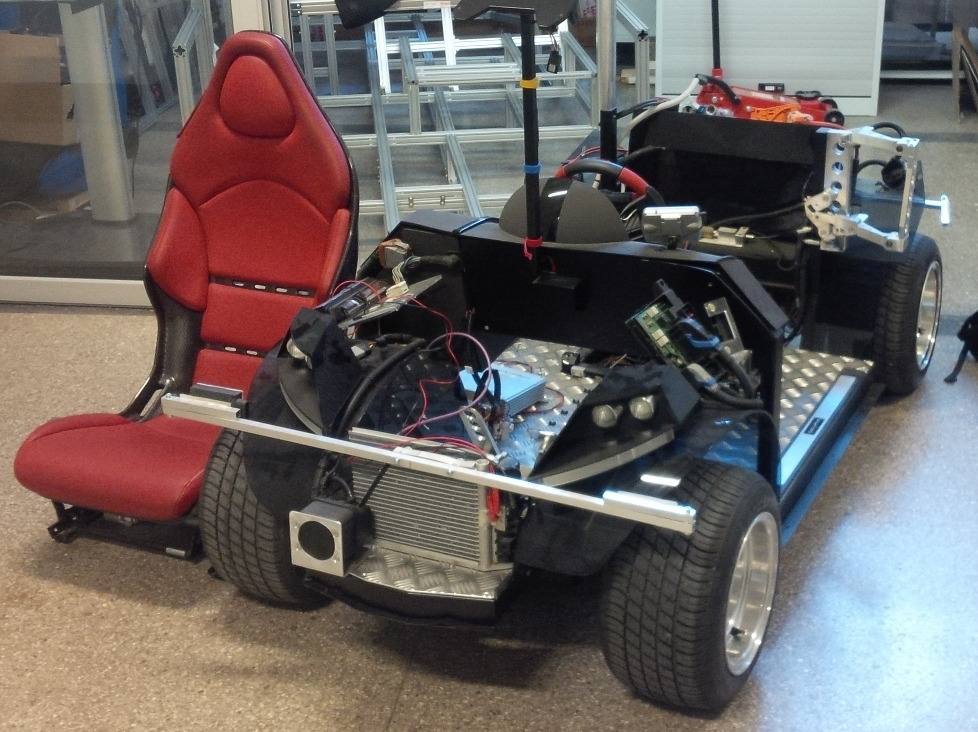
\includegraphics[scale=0.4]{pics/electric_vehicle_scaled.jpg}
	\caption{\label{fig:electric_vehicle}Samochód elektryczny udostępniony przez firmę Delphi (zdjęcie: P. Banaszkiewicz).}
\end{figure}

Awaryjne przerwanie jazdy samochodu powinno odbyć się poprzez wyłączenie zasilania silnika samochodu. O ile jest to możliwe, należy uniknąć odłączenia zasilania reszty samochodu (np. układu kierowniczego lub komputera pokładowego).

%---------------------------------------------------------------------------

\section{Cele projektu}
\label{sec:cele_projektu}

System ESAV (ang. \textit{Emergency Stop Autonomous Vehicle} – zdalny wyłącznik bezpieczeństwa dla samochodu autonomicznego) powinien charakteryzować się następującymi właściwościami:

\begin{itemize}
\item Możliwość natychmiastowego zatrzymania pojazdu na polecenie operatora.
\item Natychmiastowe zatrzymanie pojazdu w przypadku utraty zasilania systemu ESAV.
\item Natychmiastowe zatrzymanie pojazdu w przypadku przerwania transmisji pomiędzy modułami systemu ESAV.
\item Natychmiastowe zatrzymanie pojazdu w przypadku zakłóceń pracy systemu ESAV (na przykład w wyniku błędów transmisji).
\item Możliwość poruszania się pojazdu tylko jeśli system ESAV jest zasilany.
\item Możliwość poruszania się pojazdu tylko w przypadku rozpoczęcia prawidłowej transmisji danych \item pomiędzy modułami systemu ESAV.
\item Możliwość wyświetlenia aktualnego stanu systemu ESAV.
\end{itemize}

W niniejszym opisie projektu używane będą następujące pojęcia skrótowe:
\begin{itemize}
\item \textbf{moduł A}: bazowy moduł systemu ESAV; to z niego korzysta operator aby wyłączyć zasilanie silnika w samochodzie,
\item \textbf{moduł B}: moduł montowany w samochodzie, który odpowiedzialny jest za wyłączenie zasilania silnika,
\item \textbf{tryb awaryjny}: tryb modułu B w którym następuje odłączenie zasilania silnika samochodu.
\end{itemize}

Zasilanie obydwu modułów powinno być całkowicie niezależne od zasilania pojazdu, a wymianę akumulatorów łatwa. Ponadto obydwa moduły muszą monitorować i pokazywać poziom naładowania swoich akumulatorów.

Po wyłączeniu pojazdu przez system ESAV układ musi zostać przywrócony do pracy poprzez zresetowanie.

System ESAV powinien być systemem bezobsługowym: raz skonfigurowany ma poprawnie pracować bez ingerencji użytkownika. Budowa systemu powinna umożliwiać innym osobom kontynuowanie prac nad nim. W tym celu jego oprogramowanie powinno być otwarto-źródłowe, a sprzęt wymienialny.

%---------------------------------------------------------------------------

\section{Wymagania funkcjonalne}
\label{sec:wymagania_funkcjonalne}

Na podstawie opisu z rozdziału \ref{sec:cele_projektu} wyznaczono poniższe cele funkcjonalne systemu ESAV:

\begin{enumerate}[label=1.2.\arabic*:]
\item Moduł B przy braku zasilania ma odcinać zasilanie silnika samochodu.
\item Po włączeniu moduł B ma oczekiwać na dane aktywujące jego pracę, które ma otrzymać od modułu A. Stan modułu B sygnalizowany jest migającą czerwoną diodą.
\item Dopóki moduł B nie odbierze danych aktywujących, pojazd nie może się poruszać.
\item Po odebraniu danych aktywujących, moduł B powinien umożliwić jazdę samochodu. Stan modułu B sygnalizowany jest świecącą zieloną diodą.
\item Jeżeli podczas działania moduł B przestanie odbierać transmisję, musi on przejść w tryb awaryjny. Stan modułu sygnalizowany jest ciągle świecącą się czerwoną diodą.
\item Po naciśnięciu przycisku wyłączenia awaryjnego w module A przez operatora, moduł B musi przejść w tryb awaryjny. Stan modułu sygnalizowany jest ciągle świecącą się czerwoną diodą.
\item Po zresetowaniu modułu B poprzez naciśnięcie przycisku „Reset”, moduł B powraca z trybu awaryjnego do stanu oczekiwania na dane aktywujące. Stan modułu sygnalizowany jest migającą czerwoną diodą.
\item Po wyłączeniu zasilania modułu B musi nastąpić odłączenie zasilania silnika samochodu.
\item Bateria (akumulator) modułu B może być ładowana w trakcie ładowania akumulatorów pojazdu.
\end{enumerate}

%---------------------------------------------------------------------------

\section{Wymagania użytkowe}
\label{sec:wymagania_wydajnosciowe}

Na podstawie opisu z rozdziału \ref{sec:cele_projektu} wyznaczono poniższe cele zasięgu, czasu oraz szybkości działania systemu ESAV:

\begin{enumerate}
\item System ESAV musi pracować bez konieczności wymiany bądź ładowania baterii (akumulatorów) przez minimum 5 godzin.
\item System ESAV musi być w stanie co 1 sekundę odbierać i dekodować dane, a następnie je wysyłać.
\item System ESAV musi pracować poprawnie na dystansie 100 metrów w otwartej przestrzeni.
\item System ESAV musi pracować poprawnie w pomieszczeniach.
\end{enumerate}

%---------------------------------------------------------------------------

\section{Wymagania współdziałania}
\label{sec:wymagania_wspoldzialania}

Na podstawie opisu z rozdziału \ref{sec:cele_projektu} wyznaczono poniższe cele integracji systemu ESAV z innymi urządzeniami:

\begin{enumerate}
\item Moduł B musi poprawnie wyłączać silnik samochodu.
\item Moduł B powinien mieć układ ładujący podłączony do systemu elektrycznego pojazdu.
\end{enumerate}

%---------------------------------------------------------------------------

\section{Wymagania bezpieczeństwa}
\label{sec:wymagania_bezpieczenstwa}

Na podstawie opisu z rozdziału \ref{sec:cele_projektu} wyznaczono poniższe wymagania bezpieczeństwa przy korzystaniu z systemu ESAV:
\begin{enumerate}
\item Moduł B systemu ESAV nie może doprowadzić do porażenia użytkownika prądem.
\item Komunikacja pomiędzy modułami powinna zabezpieczać przed atakami powtórzenia poleceń operatora.
\item Moduł B systemu ESAV nie może nagrzewać się powyżej temperatury $50\,^{\circ}\mathrm{C}$.
\end{enumerate}

%---------------------------------------------------------------------------

\section{Wymagania pochodne}
\label{sec:wymagania_pochodne}

Wymagania, które nie zostały jawnie wspomniane w rozdziałach \ref{sec:wymagania_funkcjonalne}—\ref{sec:wymagania_bezpieczenstwa}, a wynikają albo z opisu projektu (rozdział \ref{sec:cele_projektu}), albo pojawiły się w momencie implementowania projektu, zostały opisane w tym rozdziale.

Moduł B musi:

\begin{enumerate}
\item monitorować poziom naładowania (napięcie) na baterii zasilającej,
\item sygnalizować włączenie trybu awaryjnego świeceniem czerwonej diody,
\item sygnalizować oczekiwanie na transmisję miganiem czerwonej diody,
\item sygnalizować poprawne działanie świeceniem zielonej diody.
\end{enumerate}

Moduł A musi:

\begin{enumerate}
\setcounter{enumi}{4}
\item monitorować poziom naładowania (napięcie) na baterii zasilającej,
\item sygnalizować wysyłanie informacji miganiem zielonej diody,
\item mieć małe wymiary (aby możliwe było trzymania go w dłoniach).
\end{enumerate}

Komunikacja między modułami powinna umożliwiać wymianę takich informacji:

\begin{enumerate}
\setcounter{enumi}{7}
\item PING: wymiana danych co około sekundę (do weryfikacji istnienia połączenia),
\item STOP: do wysłania danych w celu natychmiastowego przejścia modułu B w tryb awaryjny,
\item DATA: do wymiany danych diagnostycznych (np. napięcia baterii).
\end{enumerate}


%---------------------------------------------------------------------------

\section{Podsumowanie}
\label{sec:wstep_podsumowanie}

Podejście do projektu oparte o listę wymagań (ang. \textit{requirements-driven design} \cite{Hug10} albo \textit{feature-driven development} \cite{Goy08}) umożliwia sprecyzowanie niewielkich wymagań a priori, które pozwalają wykonawcy implementować funkcjonalności pojedyncze i skierowane na konkretne wymagania, a także śledzić spełnienie tych wymagań w formie prostej tabeli (zob. rozdział \ref{sec:zrealizowane_wymagania}).

W tym rozdziale zostały wyszczególnione wymagania według sugerowanego schematu z~\cite{Hug10}, jednakże w przypadku projektów stricte programistycznych schemat ten może wyglądać inaczej.

Skupienie się na wyszczególnieniu wymagań przed rozpoczęciem prac nad projektem znacząco ułatwiło jego tworzenie, m.in. poprzez eliminację luk w opisie funkcjonalnym systemu ESAV.

%% Może warto by dodać rysunek poglądowy, samochód, osoba trzymająca wyłącznik - tak żeby było widać, że nie jest to zwykły wyłącznik ale coś więcej.

\chapter{Specyfikacja projektu}
\label{cha:specyfikacja_projektu}

W tym rozdziale opisane zostało wykonanie projektu zgodnie z wymaganiami postawionymi w rozdziale \ref{cha:wstep}.

%---------------------------------------------------------------------------

\section{Opis części sprzętowej}
\label{sec:opis_cz_sprzetowej}

W poniższym rozdziale została opisana platforma sprzętowa modułów A i B oraz ich współdziałanie z innymi komponentami, m.in. z zasilaniem akumulatorowym czy z przekaźnikiem w samochodzie elektrycznym.

\subsection{Moduł A}
\label{subsec:modul_a}

Jest to moduł bazowy, tj. trzymany przez operatora w dłoni. Ze względu na użycie Arduino Pro 328 5V 16MHz \cite{Ard00} (zob. zdjęcie \ref{fig:arduino_pro}) jako platformy sprzętowej, ma on niewielkie wymiary.

\begin{figure}[h]
	\centering
	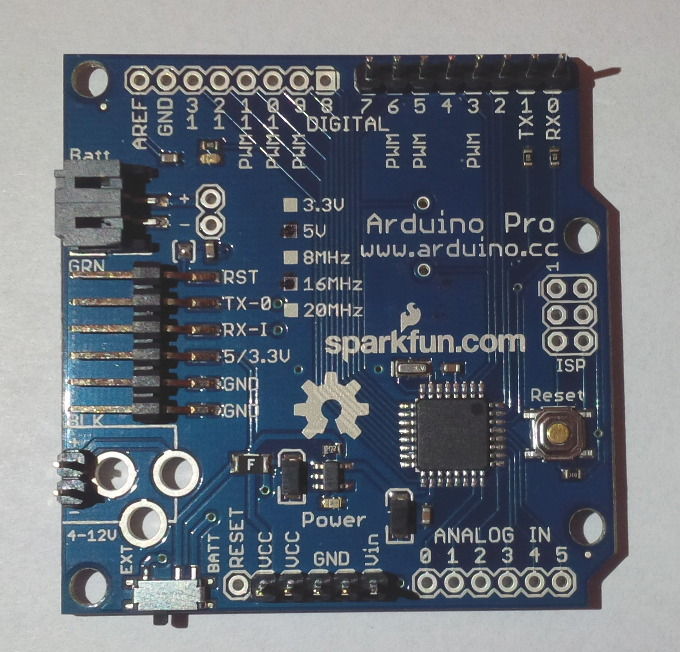
\includegraphics[scale=0.3]{pics/arduino_pro_scaled.jpg}
	\caption{\label{fig:arduino_pro}Platforma sprzętowa Arduino Pro 328 5V 16MHz (zdjęcie: Piotr Banaszkiewicz).}
\end{figure}

\subsection{Moduł B}
\label{subsec:modul_b}

Jest to moduł, który został zamontowany w samochodzie. Jako platformę użyte zostało ponownie Arduino Pro 328 5V 16MHz \cite{Ard00} (zob. zdjęcie \ref{fig:arduino_pro}). Podstawowa funkcja, tj. odłączanie i załączanie silnika elektrycznego, odbywa się za pomocą przekaźnika ASR-90DD-H firmy Anly Electronics (zob. zdjęcie \ref{fig:SSR_relay} i rozdział \ref{subsec:odlaczanie_zalaczanie_silnika}).

\begin{figure}[h]
	\centering
	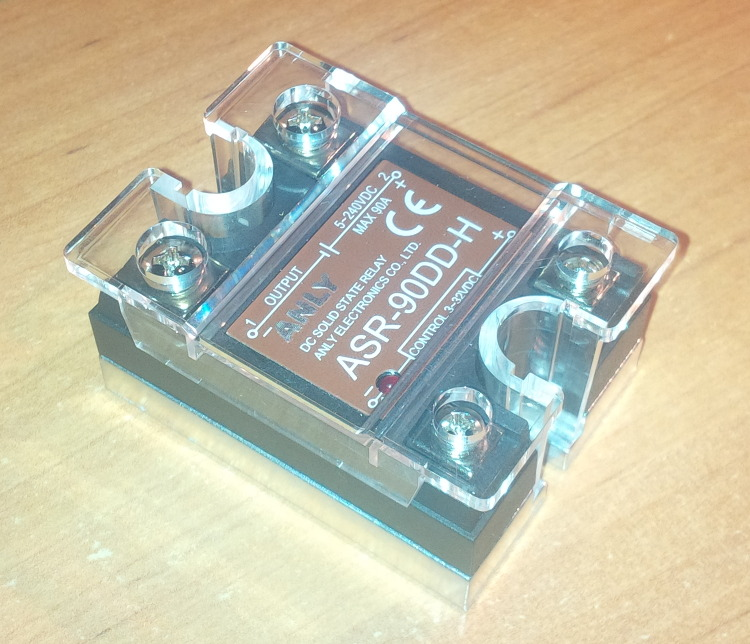
\includegraphics[scale=0.3]{pics/Anly_ASR90DDH.jpg}
	\caption{\label{fig:SSR_relay}Przekaźnik półprzewodnikowy ASR-90DD-H  (zdjęcie: Piotr Banaszkiewicz).}
\end{figure}

\subsection{Zasilanie}
\label{subsec:zasilanie}

Obydwa moduły sprzętowe są zasilane z powerbanków Solo5 10000 mAh firmy Romoss. Posiadają one wbudowane różne zabezpieczenia, m.in.: natężeniowe (dla zachowania żywotności), temperaturowe czy zwarciowe (ang. \textit{short-circuit}). Mają również układ, który wyłącza powerbank w sytuacji, gdy prąd ładowania jest bardzo niewielki.  %% DODAJ BIBLIO?

Moduły A i B pobierają bardzo niewiele prądu (zmierzone: między 20 a 50 mA), więc aby powstrzymać powerbanki przed rozłączaniem zwarto masę i źródło energii dwunastoma (w przypadku modułu A) lub trzynastoma (w przypadku modułu B) rezystorami $ 910 \Omega $ wpiętymi równolegle.

Połączenie równoległe takiej ilości rezystorów daje dość niską rezystancję zastępczą (teoretycznie: $ 75.83 \Omega $ dla modułu A, $ 70 \Omega $ dla modułu B; praktycznie: występują różnice w faktycznych wartościach rezystancji rezystorów, zwłaszcza gdy te się nagrzeją) i pozwala na obniżenie wydzielanego ciepła na rezystorach, co skutkuje:

\begin{itemize}
\item większym poborem prądu, dzięki czemu powerbanki się nie wyłączają,
\item nagrzewaniem rezystorów (z prawa Ohma: $ P = \dfrac{U^2}{R} = \dfrac{(5.1)^2}{900} = 0.0289 [W] $, gdzie $ 5.1 [V] $ to zmierzone napięcie na rezystorze, a $ 900 [\Omega] $ to przybliżona rezystancja nagrzanego rezystora), a więc w przypadku 12 rezystorów położonych bardzo blisko siebie mamy około $ 0.34 [W] $ wydzielanej mocy w tym miejscu.
\end{itemize}

Ponadto banki energii umożliwiają jednoczesne ładowanie jak i rozładowywanie, tzn. jest możliwe wpięcie źródła zasilania na wejście powerbanku, jak i obciążenia na jego wyjście. Dzięki temu powerbank zasilający moduł B można ładować z portu USB znajdującego się w~samochodzie.

Sama pojemność 10000mAh teoretycznie\footnote{W praktyce pojemność 10000mAh jest nieosiągalna, gdyż powerbanki posiadają mechanizmy wydłużające ich żywotność; polega to na ładowaniu akumulatorów powerbanku tylko do pewnego stopnia.} pozwala na zasilanie układu pobierającego 100mA przez 100 godzin lub układu pobierającego 200mA przez 50 godzin. Każdy z modułów A i B po obciążeniu przez rezystory pobierał między 100 a 200 mA. Poziom naładowania powerbanków można obserwować na ich diodowych wskaźnikach.

\subsection{Komunikacja}
\label{subsec:komunikacja}

Do komunikacji wykorzystano parę modułów radiowych HC-12 433 MHz \cite{HC12}, które łączą się z~platformami sprzętowymi za pomocą łącza szeregowego. Prędkość komunikacji takiego modułu w powietrzu wynosi 5000bps, czyli typowe pakiety przesyłane przez system (zob. rozdział \ref{subsec:format_pakietow}), mające rozmiar $ 4B=32b $ są przesyłane w ułamku sekundy.

\subsection{Obudowy i montaż}
\label{subsec:obudowy_montaz}

Dla każdego modułu została zaprojektowana obudowa. Na zdjęciu \ref{fig:arduino_pro} widać cztery otwory w platformie Arduino (dwa przy lewej krawędzi płytki PCB oraz dwa przy prawej krawędzi), które zostały użyte do przykręcenia każdej z platform do obudowy.

Ponadto na każdą platformę Arduino przygotowano nakładaną na piny płytkę uniwersalną z~przylutowanymi komponentami wykorzystywanymi przez dany moduł.  %% DODAJ ZDJĘCIE PŁYTEK UNIWERSALNYCH

Obudowy zostały wydrukowane w drukarce 3D.  %% DODAJ ZDJĘCIE PROJEKTÓW OBUDÓW

\subsection{Schematy połączeń}
\label{subsec:schematy_polaczen}

Symboliczny sposób połączenia modułu A, wejścia zasilającego USB oraz transceivera radiowego został przedstawiony na schemacie \ref{fig:symbolic_schema_A}.

\begin{figure}[H]
	\centering
	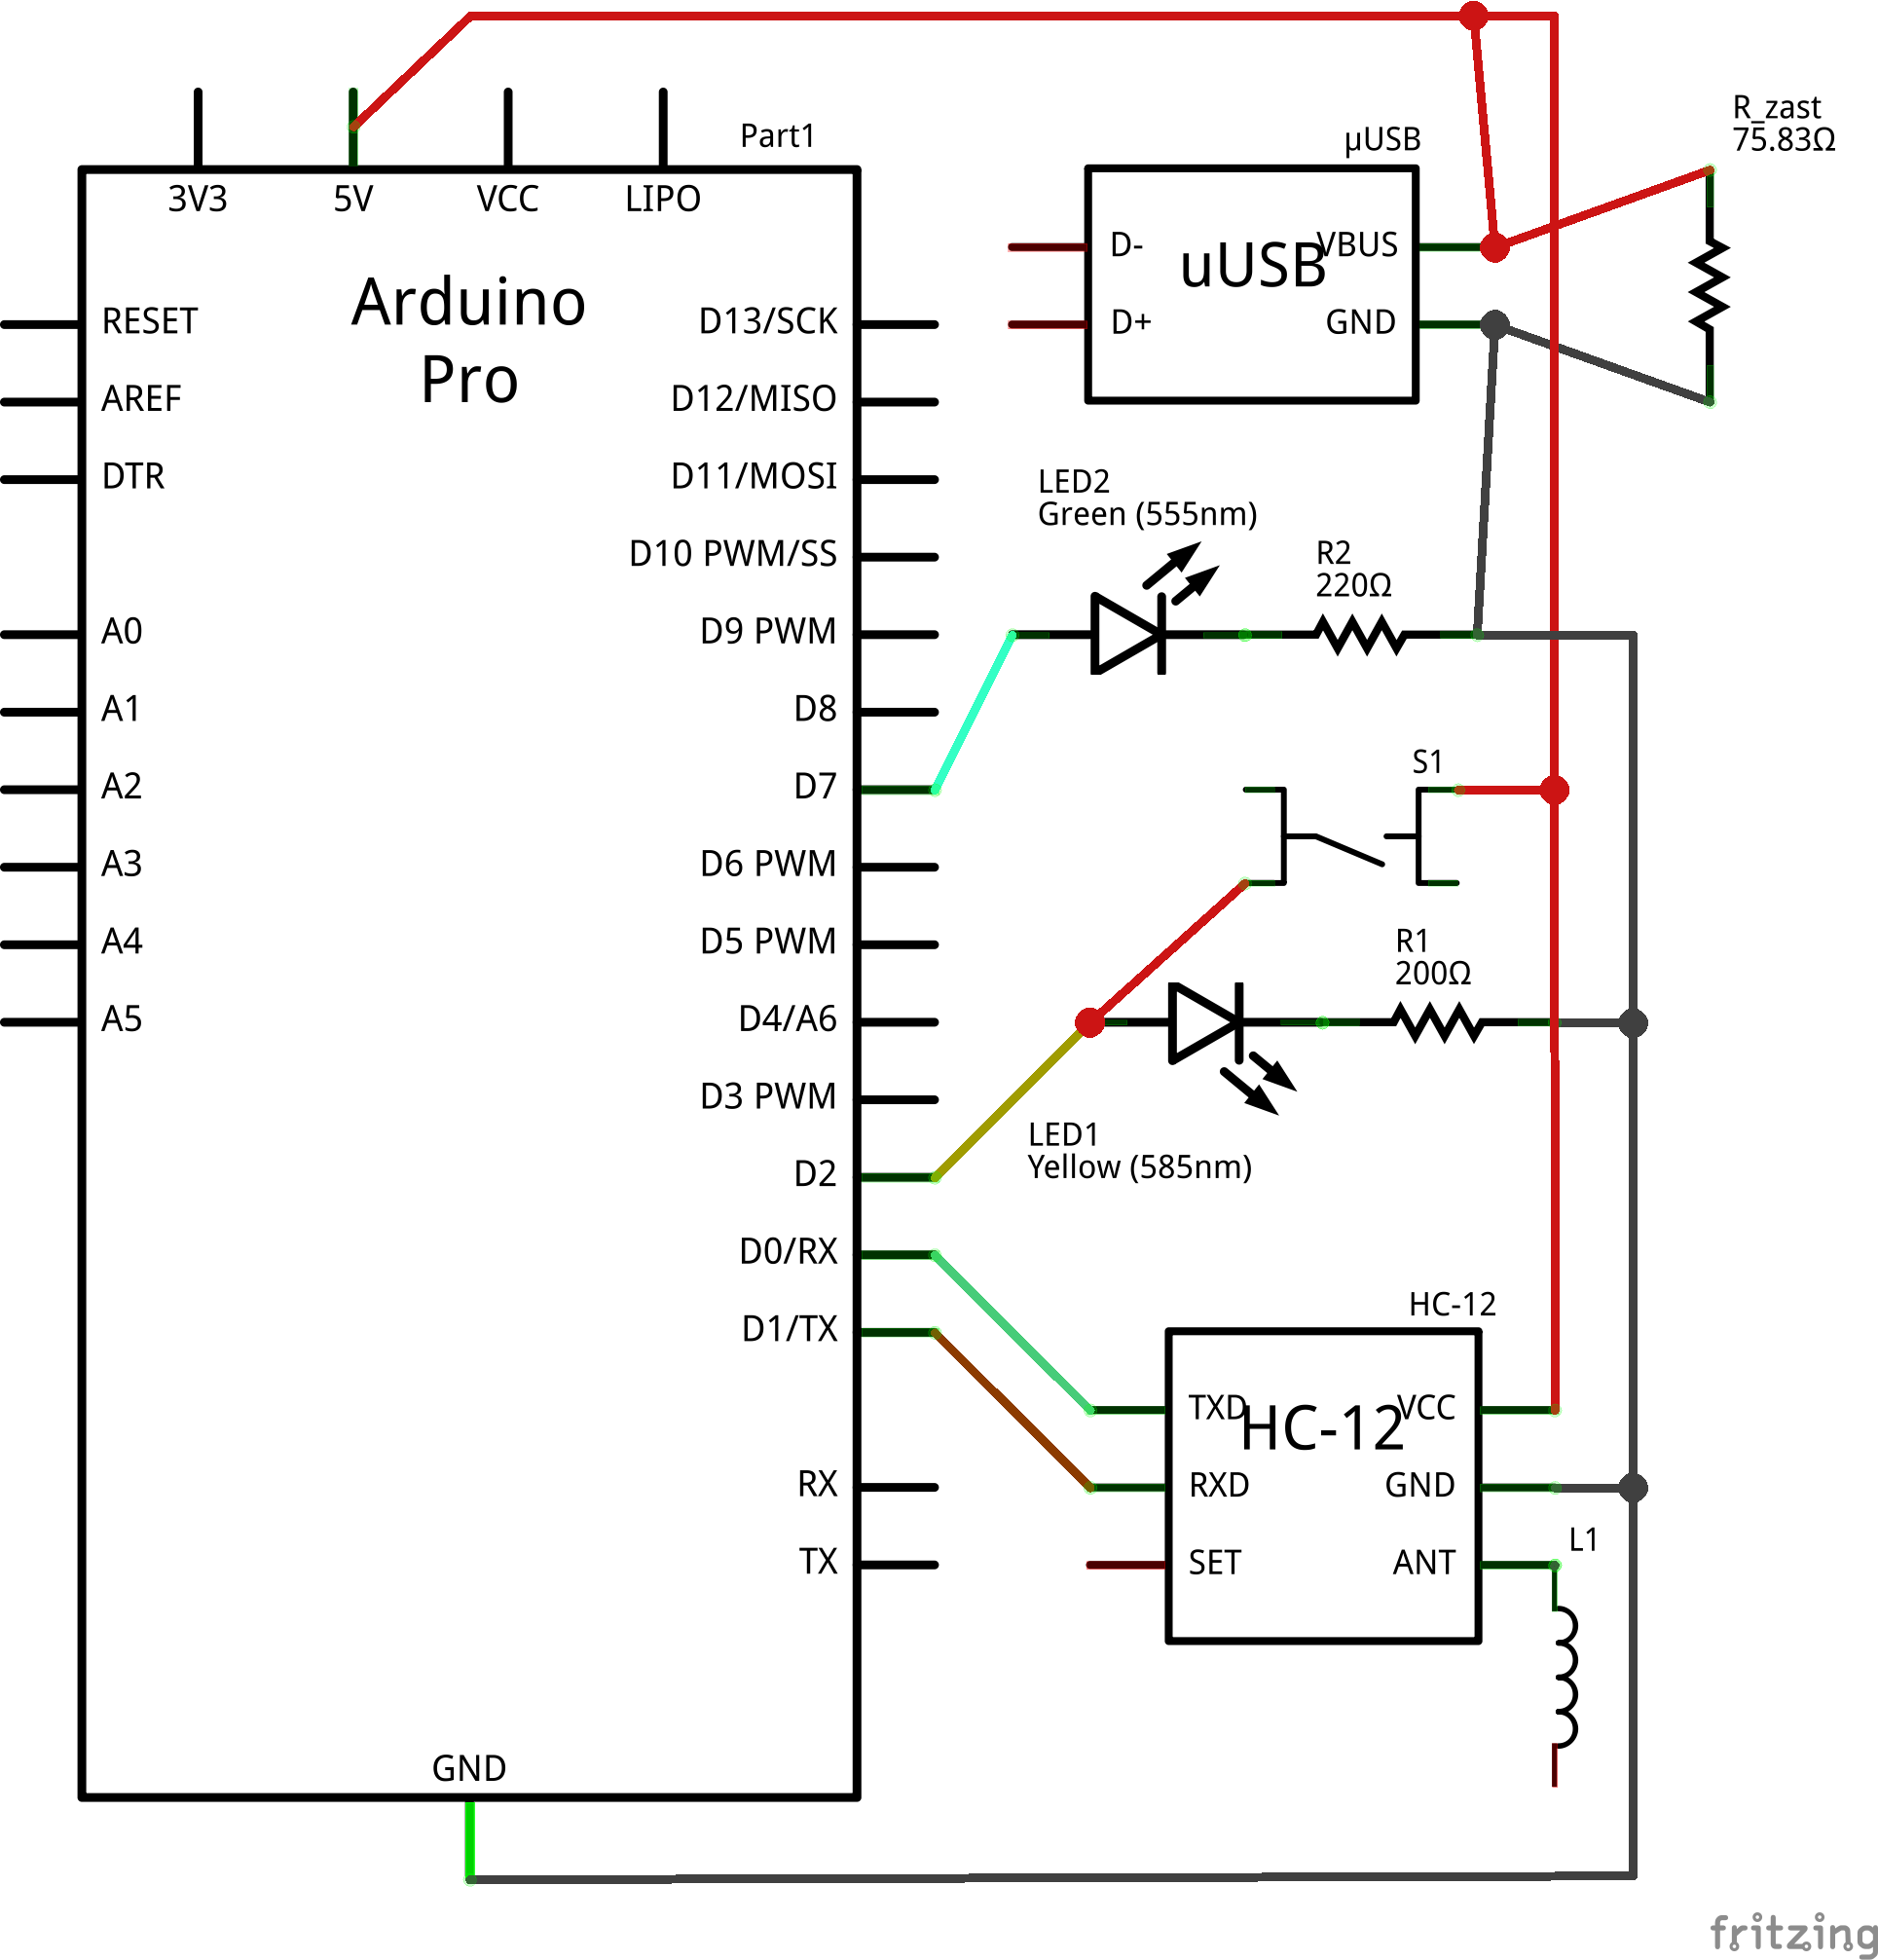
\includegraphics[scale=0.4]{schemas/schema_moduleA_schem.png}
	\caption{\label{fig:symbolic_schema_A}Schemat połączeń modułu A wygenerowany w programie Fritzing \cite{Fritzing} (opracowanie własne).}
\end{figure}

Bardzo podobnie wygląda symboliczny schemat połączeń modułu B, z tym że on dodatkowo steruje przekaźnikiem (schemat \ref{fig:symbolic_schema_B}).

\begin{figure}[H]
	\centering
	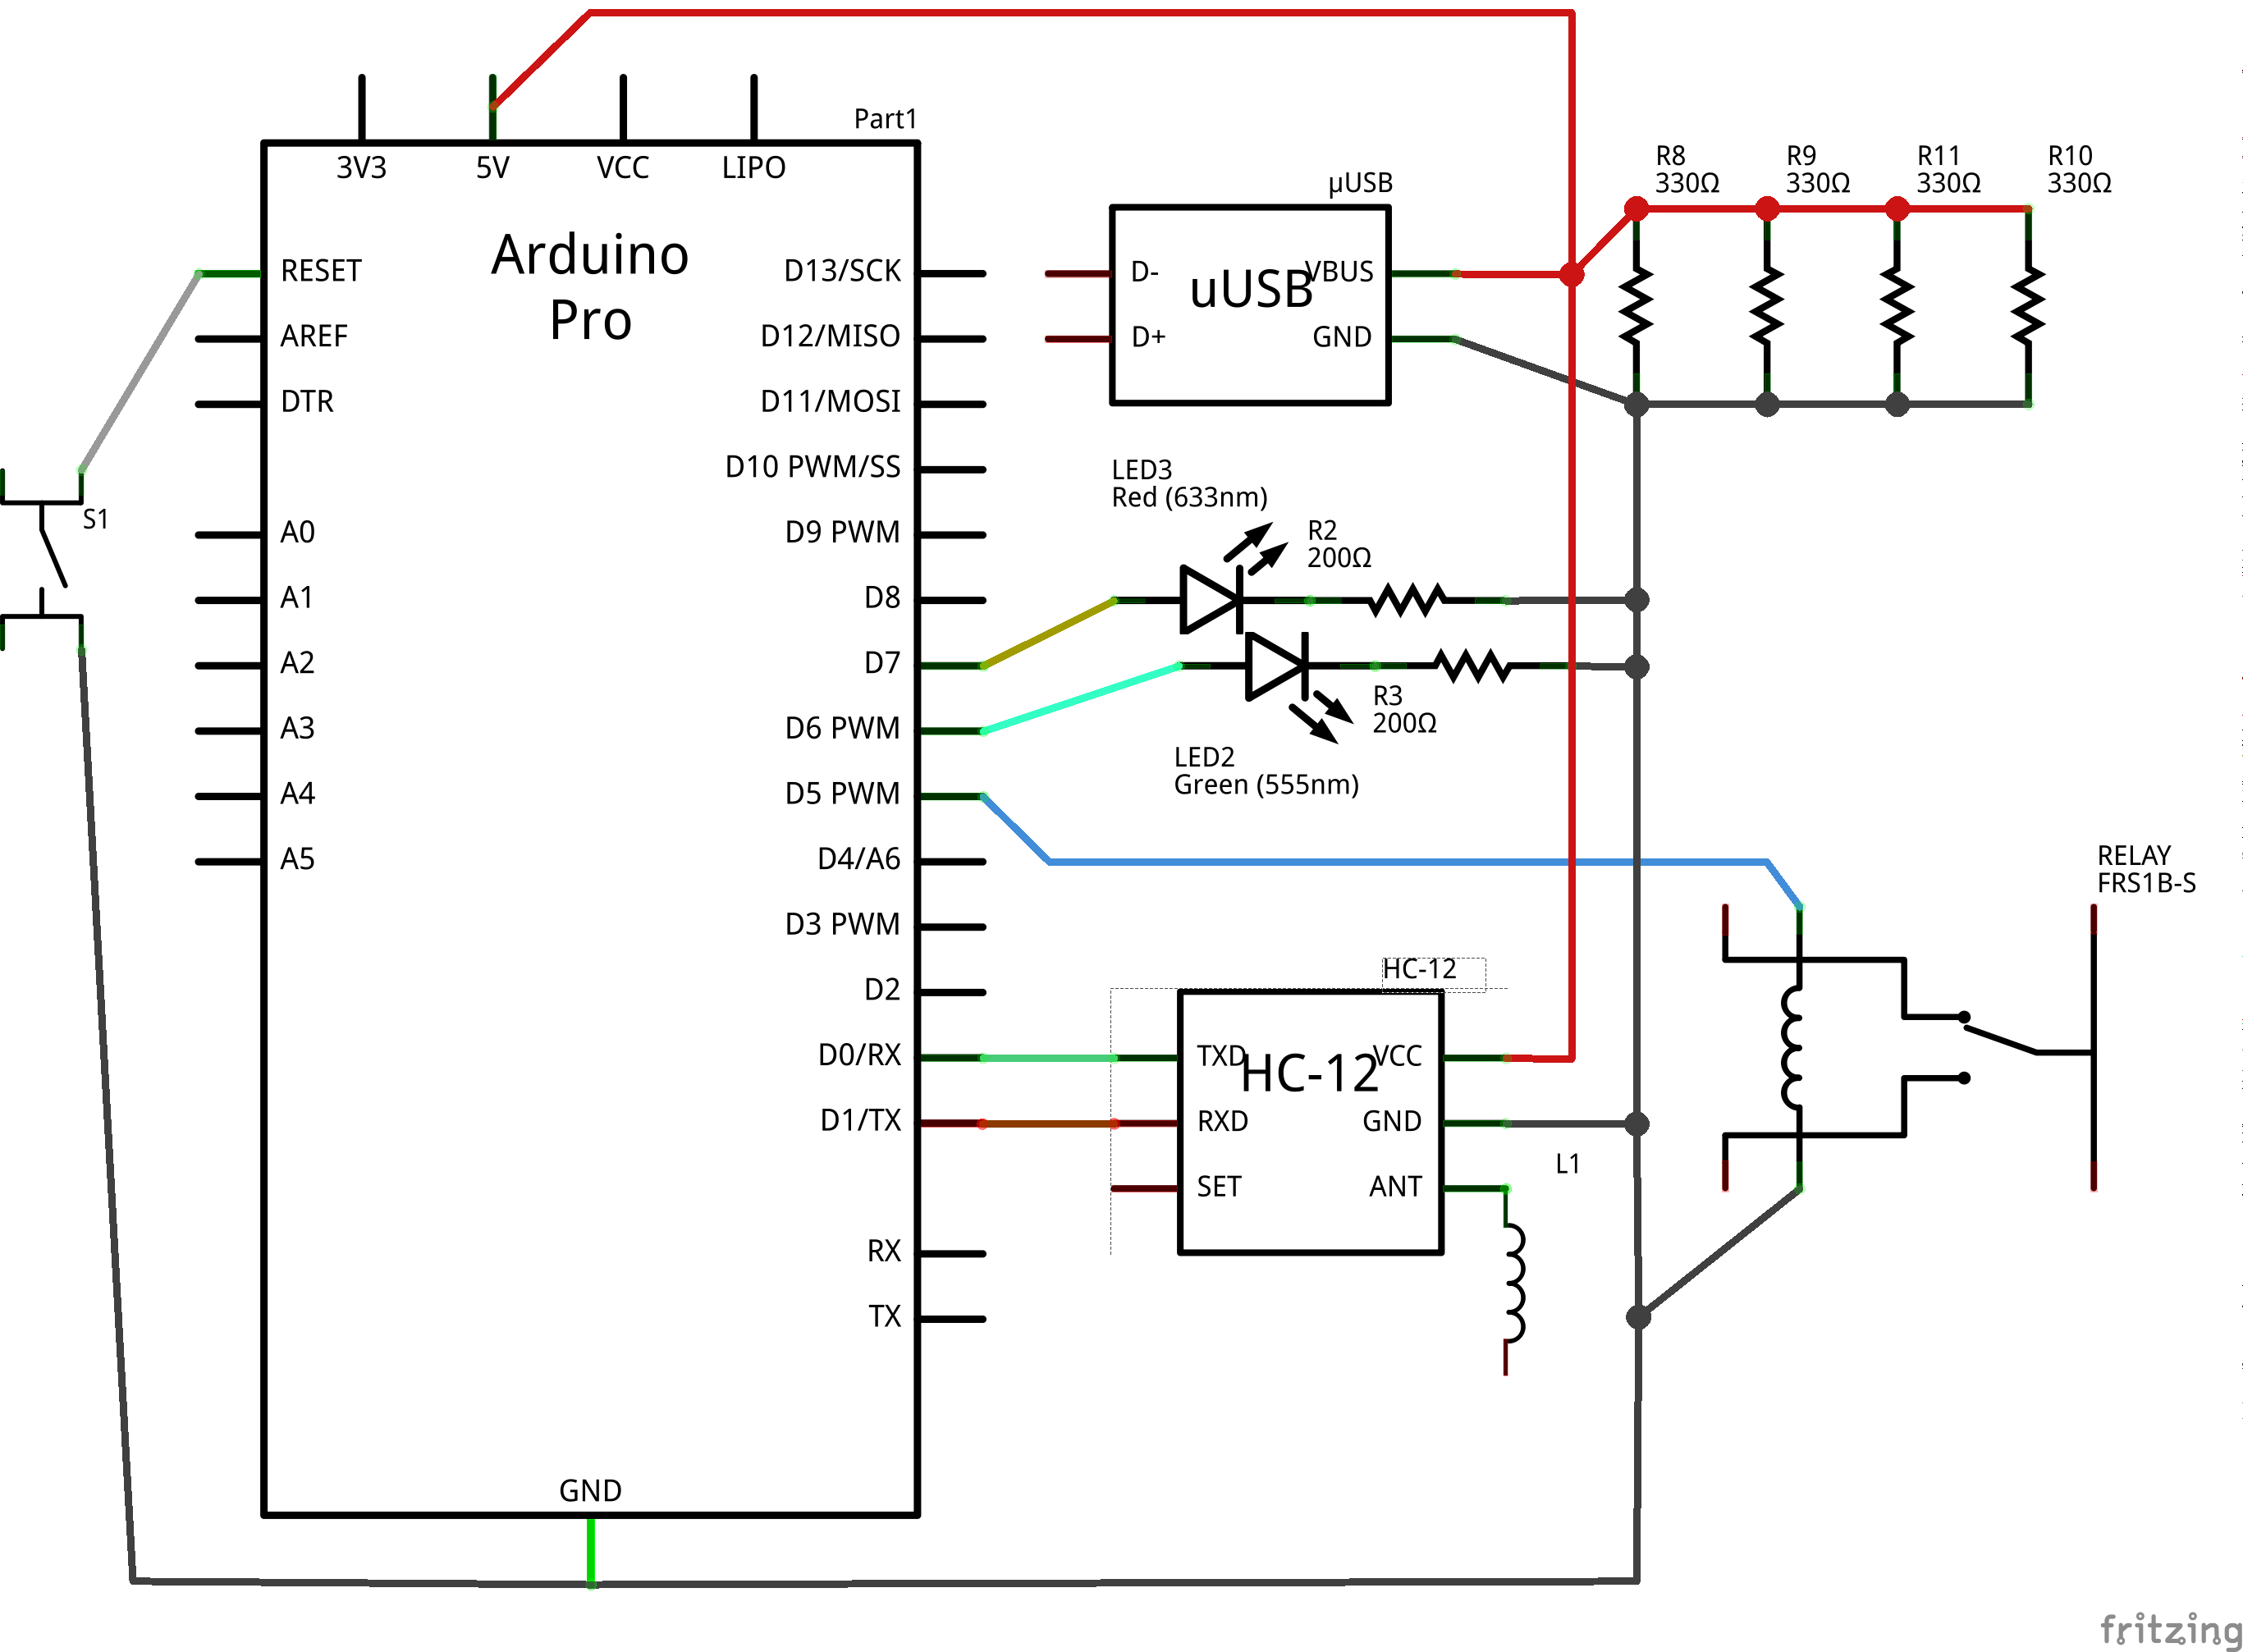
\includegraphics[scale=0.4]{schemas/schema_moduleB_schem.png}
	\caption{\label{fig:symbolic_schema_B}Schemat połączeń modułu B wygenerowany w programie Fritzing \cite{Fritzing} (opracowanie własne).}
\end{figure}

\subsection{Odłączanie i załączanie silnika samochodu}
\label{subsec:odlaczanie_zalaczanie_silnika}

Pomiędzy kabel zasilający a moduł sterujący pracą silnika samochodu został wpięty przekaźnik ASR-90DD-H (zob. zdjęcie \ref{fig:SSR_relay}). Moduł sterujący odpowiedzialny jest za przetworzenie napięcia stałego na prąd zmienny poprowadzony bezpośrednio na uzwojenia silnika.

Przekaźnik ASR-90DD-H jest to przekaźnik półprzewodnikowy sterowany napięciem 3–32VDC, a zatem typu \textit{Normally Open}. Przekaźnik jest sterowany wyjściem z modułu B (zob. element ,,RELAY'' na schemacie \ref{fig:symbolic_schema_B}).

Według danych producenta, przekaźnik jest w stanie obsłużyć na wyjściu mocy do 90A prądu stałego pod napięciem do 240V. Wybrano przekaźnik mocno przekraczający spodziewane natężenie prądu, gdyż zapewnia to mniejsze wydzielanie ciepła (zob. rozdział \ref{subsec:chlodzenie_SSR}).

Niestety producent nie udostępnia schematu elektrycznego przekaźnika w dokumentacji \cite{ASR90DDH}, więc podczas jego montażu zadbano o kilka elementów bezpieczeństwa:

\begin{itemize}
\item zastosowano podkładkę silikonową jako izolator elektryczny,
\item zastosowano radiator chłodzący (widoczny na zdjęciu \ref{fig:radiator}).
\end{itemize}

\begin{figure}[h]
	\centering
	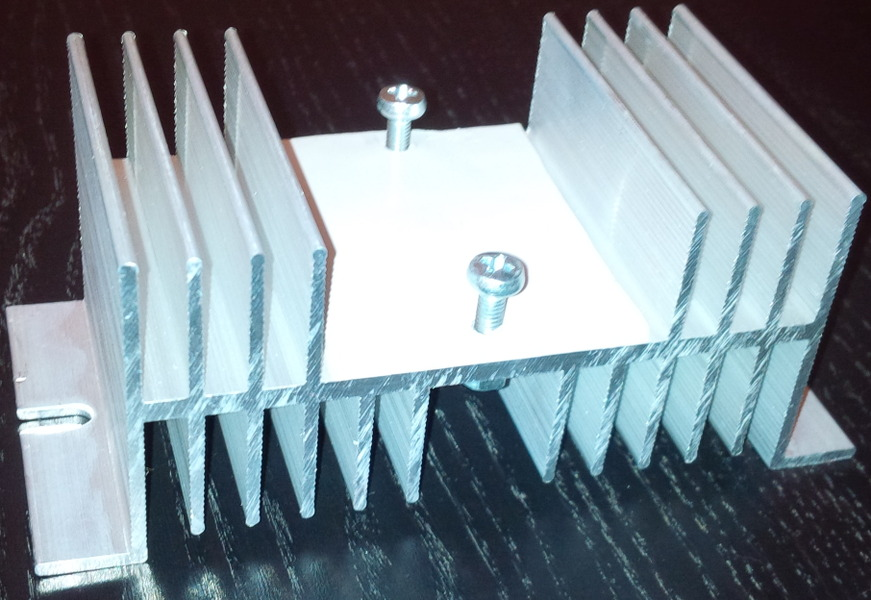
\includegraphics[scale=0.35]{pics/radiator.jpg}
	\caption{\label{fig:radiator}Radiator chłodzący przekaźnik SSR (zdjęcie: Piotr Banaszkiewicz).}
\end{figure}

Elementy te zgodne są z zaleceniami polskiego producenta przekaźników, firmy Relpol \cite{RELPOL}.

\subsection{Chłodzenie przekaźnika półprzewodnikowego}
\label{subsec:chlodzenie_SSR}

Przekaźniki półprzewodnikowe z powodu pewnej niskiej oporności własnej w momencie podłączonego wyjścia mocy wydzielają dużą ilość energii w postaci ciepła.

W ramach pracy inżynierskiej przeprowadzono eksperyment polegający na zmierzeniu temperatury obudowy działającego przekaźnika podczas włączonego obciążenia.

Przekaźnik został umieszczony na radiatorze i pracował przez kilka minut (do momentu ustalenia się temperatury) pod stałym obciążeniem. Kamera termowizyjna ostawiona była tak, by mierzyć temperaturę radiatora oraz obudowy przekaźnika. Tabela \ref{tab:eksperyment} zawiera zestawienie długości czasu działania przekaźnika pod obciążeniem, a także uzyskanej na końcu eksperymentu temperatury, natomiast zdjęcia 5 i 6 ukazują obrazy z kamery termowizyjnej.  %% Linki do tabeli oraz zdjęć

\begin{table}[h]
    \centering
    
    \begin{threeparttable}
        \caption{Parametry eksperymentu obciążenia przekaźnika półprzewodnikowego}
        \label{tab:eksperyment}
        
        \begin{tabularx}{0.9\textwidth}{cccXX}
            \toprule
            Czas obciążenia [min] & Napięcie [V] & Natężenie [A] & Temperatura radiatora\tnote{a} [\degree C] & Temperatura obudowy przekaźnika\tnote{a} [\degree C] \\
            \midrule
            8 & 45 & 36 & 25 & ok. 60 \\
            8 & 42.5 & 43 & 25 -- 35 & ok. 90 \\
            \bottomrule
        \end{tabularx}
        
        \begin{tablenotes}
            \footnotesize
            \item[a] pod koniec pomiaru
        \end{tablenotes}
        
    \end{threeparttable}
\end{table}

\begin{figure}[H]
	\centering
	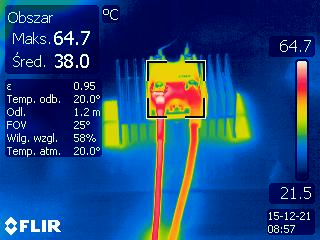
\includegraphics[scale=0.8]{flir/IR_5167.jpg}
	\caption{\label{fig:flir1}Obraz uzyskany za pomocą kamery termowizyjnej na koniec trwania eksperymentu z mniejszym obciążeniem (zdjęcie: Marek Długosz).}
\end{figure}

\begin{figure}[H]
	\centering
	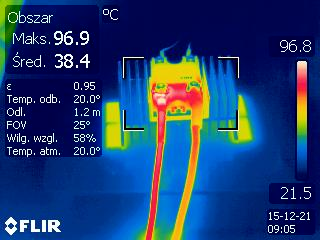
\includegraphics[scale=0.8]{flir/IR_5170.jpg}
	\caption{\label{fig:flir1}Obraz uzyskany za pomocą kamery termowizyjnej na koniec trwania eksperymentu z większym obciążeniem (zdjęcie: Marek Długosz).}
\end{figure}

Na powyższych zdjęciach najcieplejszym elementem była śruba służąca do przykręcenia kabla zasilającego. Temperatura ciepłego miejsca na obudowie przekaźnika była o około $ 15^{\circ}\mathrm{C} $ niższa; uwzględnione to zostało w tabeli \ref{tab:eksperyment} poprzez odjęcie ok. $ 10^{\circ}\mathrm{C} $ od maksymalnej mierzonej temperatury.

Ponadto należy zauważyć jak niewiele nagrzewał się radiator, do którego przymocowany został przekaźnik. To udowadnia, że jest on wystarczający dla zastosowania w samochodzie.

Na samym końcu należy zauważyć, że przekaźnik nie powinien być w realnych zastosowaniach narażony na tak duże obciążenia przez tak długi czas; według obserwacji, pobór maksymalny chwilowy w trakcie przyspieszania pojazdu i skręcania jednocześnie wynosił około $ 50A $.

%---------------------------------------------------------------------------

\section{Opis części programowej}
\label{sec:opis_cz_programowej}

W tym rozdziale opisano m.in. logikę, algorytmy i struktury danych wykorzystywane przez programy modułów A i B.

\subsection{Schematy cykli-działań}
\label{subsec:schematy_cykli_dzialan}

Poniższe schematy reprezentują logikę, zdarzenia oraz czynności, jakimi posługują się moduły A~i~B.

Dokładny opis pakietów danych oraz momenty, w których są przesyłane, znajduje się w rozdziale \ref{subsec:format_pakietow}.

\raggedbottom

\begin{figure}[H]
	\centering
	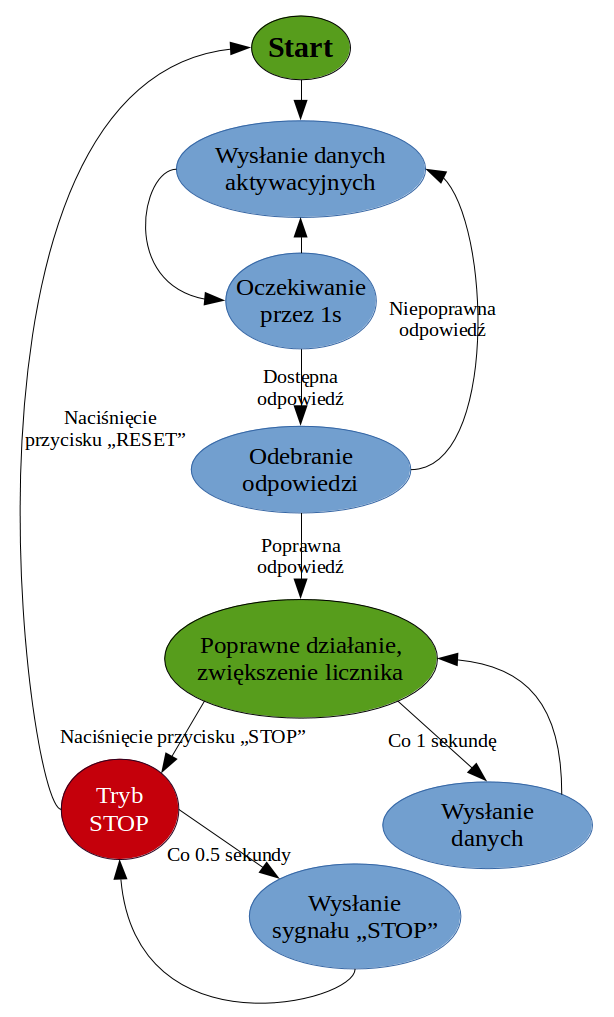
\includegraphics[scale=0.8]{schemas/cycle_action_A.png}
	\caption{\label{fig:cycle_action_A}Graf cykli-działań dla modułu A (opracowanie własne).}
\end{figure}

\begin{figure}[H]
	\centering
	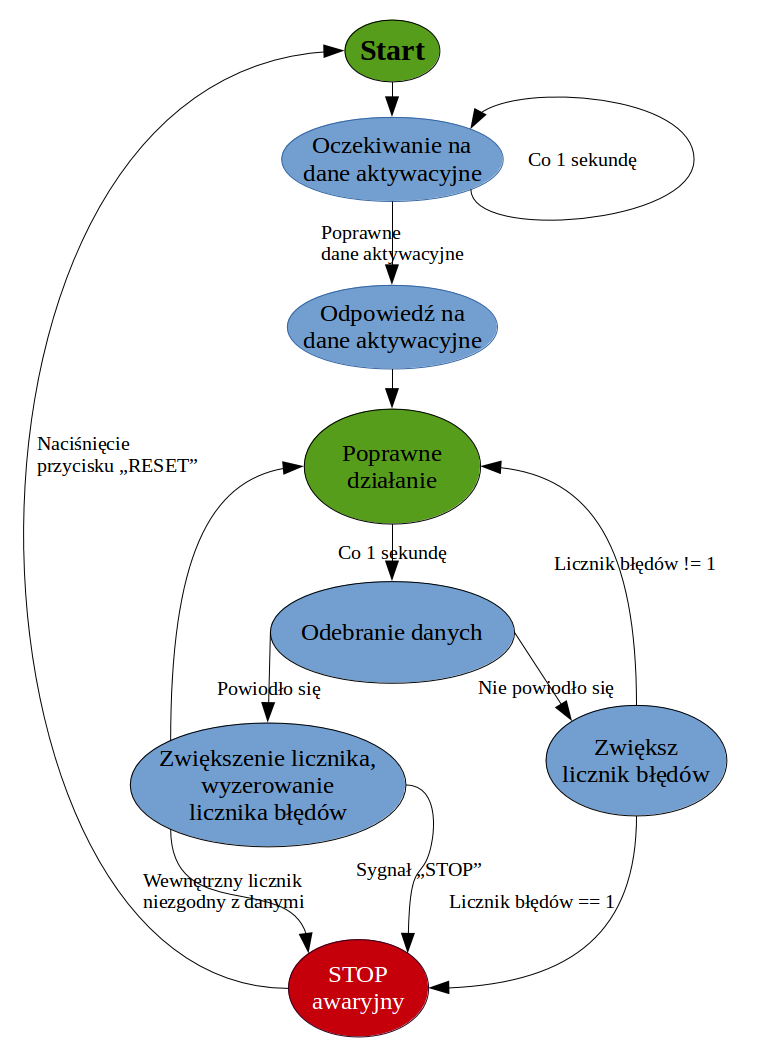
\includegraphics[scale=0.8]{schemas/cycle_action_B.png}
	\caption{\label{fig:cycle_action_B}Graf cykli-działań dla modułu B (opracowanie własne).}
\end{figure}

\subsection{Format pakietów}
\label{subsec:format_pakietow}

Każdy pakiet ma długość 4 bajtów:

\begin{equation}
0 \mathrm{x} \underbrace{\mathrm{FC}}_\text{e}  \underbrace{\mathrm{ABCD}}_\text{c} \underbrace{00}_\text{s}
\end{equation}
gdzie
\begin{eqwhere}[2cm]
	\item[$e$] bajt \textit{emergency}. Jeżeli jego wartość to $0xFF$ to moduł B ma natychmiast przejść do trybu awaryjnego. W praktyce oznacza to, że operator wcisnął przycisk ,,STOP'' modułu A.
	\item[$c$] 2 bajty zapisujące wartość liczbową licznika modułu A (typ bez znaku, 16 bitów),
	\item[$s$] bajt stopu, jego wartość zawsze ma być równa $0x00$.
\end{eqwhere}

Istnieją 2 pakiety specjalne przesyłane między modułami A i B w celu synchronizacji i rozpoczęcia działania:

\begin{itemize}
\item pakiet danych aktywacyjnych wysyłany przez moduł A: $0\mathrm{xFFFFFF}00$,
\item pakiet odpowiedzi na dane aktywacyjne wysyłany przez moduł B: $0\mathrm{x11FFFF}00$,
\item ponadto każdy pakiet danych wysyłany przez moduł A już po odebraniu odpowiedzi na dane aktywacyjne zawiera bajt \textit{emergency} ustawiony na wartość $0\mathrm{x}22$ -- za wyjątkiem sytuacji, w której moduł A żąda od modułu B przejścia w tryb awaryjny; wtedy ten bajt ustawiony jest na wartość $0\mathrm{xFF}$.
\end{itemize}

Przykładowe pakiety:

\begin{itemize}
\item $0\mathrm{x}223\mathrm{F}0\mathrm{E}00$: moduł A wysyła informację o braku konieczności przejścia w tryb awaryjny oraz o wartości licznika (16142),
\item $0\mathrm{xFFA}37800$: moduł A wysyła informację o przejściu w tryb awaryjny oraz o ostatniej wartości licznika (41848).
\end{itemize}

\subsection{Maszyna stanów}
\label{subsec:maszyna_stanow}

Oprogramowanie modułów A i B wykorzystuje proste maszyny stanów \cite{Bro69}.

Stany modułu A:

\begin{enumerate}
\item CONNECTING: wysyłanie pakietu danych aktywacyjnych co 1 sekundę, oczekiwanie na odpowiedź,
\item PING: wysyłanie obecnej wartości licznika co 1 sekundę, zwiększanie wartości licznika,
\item STOP: wysyłanie ostatniej wartości licznika oraz ustawionego bajtu \textit{emergency} co $0.5$ sekundy.
\end{enumerate}

Stany modułu B:

\begin{enumerate}
\item WAIT: oczekiwanie na przyjście pakietu danych aktywacyjnych; odesłanie na niego odpowiedzi,
\item RUN: zwiększanie wewnętrznego licznika, odbieranie wartości licznika modułu A, porównywanie obu liczników, sprawdzanie bajtu \textit{emergency},
\item STOP: podtrzymywanie wyłączenia zasilania.
\end{enumerate}

Warunki przejścia między stanami modułu A:

\begin{itemize}
\item CONNECTING $\rightarrow$ PING: gdy pakiet odpowiedzi na dane aktywacyjne wysłany przez moduł B to $0\mathrm{x}11\mathrm{FFFF}00$,
\item PING $\rightarrow$ STOP: gdy operator wciśnie przycisk ,,RESET''.
\end{itemize}

Warunki przejścia między stanami modułu B:

\begin{itemize}
\item WAIT $\rightarrow$ RUN: gdy pakiet danych aktywujących wysłany przez moduł A to $0\mathrm{xFFFFFF}00$,
\item RUN $\rightarrow$ STOP: gdy jeden z warunków jest spełniony:
    \begin{itemize}
    \item bajt \textit{emergency} w przychodzącym pakiecie ma wartość $0\mathrm{xFF}$,
    \item licznik wewnętrzny ma wartość różną od wartości licznika wysłanej przez moduł A w przychodzącym pakiecie,
    \item przez 3 sekundy nie nadeszły żadne dane od modułu A.
    \end{itemize}
\end{itemize}

\subsection{Panel operatorski}
\label{subsec:panel_operatorski}

Obydwa moduły systemu ESAV zawierają minimalny interfejs dla użytkownika. Składa się on odpowiednio z:

\begin{itemize}
\item dla modułu A:
    \begin{itemize}
    \item przycisk ,,STOP'' wywołujący przerwanie wewnętrzne platformy Arduino i w konsekwencji wysłanie polecenia przejścia do trybu awaryjnego,
    \item przycisk ,,RESET'' do łatwiejszego restartu urządzenia,
    \item zieloną diodę informującą o wysyłaniu danych przez port szeregowy,
    \item żółtą diodę włączającą się w momencie naciśnięcia przycisku ,,STOP'' (spełnia ona funkcję wizualnego sprzężenia zwrotnego dla użytkownika),
    \end{itemize}
    
\item dla modułu B:
    \begin{itemize}
    \item przycisk ,,RESET'' do łatwiejszego restartu urządzenia,
    \item zieloną diodę informującą o poprawnym trybie pracy (stan ,,RUN''),
    \item czerwoną diodę informującą o oczekiwaniu na dane wejściowe (szybka pulsacja) lub o przejściu w tryb awaryjny (ciągłe świecenie).
    \end{itemize}
\end{itemize}

\subsection{Szyfrowanie komunikacji}
\label{subsec:szyfrowanie_komunikacji}

Komunikacja pomiędzy modułami (za wyjątkiem przekazywanych danych aktywacyjnych i odpowiedzi na nie) jest w prosty sposób szyfrowana.

Do szyfrowania wykorzystywane są dwie tablice, każda o długości 256, co odpowiada ilości wartości pojedynczego bajtu. Szyfrowanie pojedynczego bajtu polega na odszukaniu w tablicy szyfrującej odpowiadającej mu wartości zaszyfrowanej, a odszyfrowanie polega na odszukaniu w tablicy deszyfrującej wartości oryginalnej odpowiadającej wartości zaszyfrowanej.

Poniższy przykład ilustruje szyfrowanie i deszyfrowanie na przykładzie czterech wartości:

\begin{lstlisting}[frame=single,caption=Pseudokod zbliżony do C pokazujący zasadę szyfrowania i deszyfrowania komunikacji systemu ESAV.]
byte cipher_array[] = {3, 1, 0, 2};
byte decipher_array[] = {2, 1, 3, 0};
byte original = 2;
byte encrypted = cipher_array[original];
assert(original == decipher_array[encrypted]);
\end{lstlisting}

Dzięki wykorzystaniu tej prostej metody nie nastąpił żaden narzut w wielkości przesyłanych pakietów, niestety skutkiem słabszego bezpieczeństwa niż w przypadku stosowania np. algorytmu AES \cite{AESComment}.

\subsection{Programowanie Arduino}
\label{subsec:programowanie_arduino}

Platforma Arduino, na której oparty jest system ESAV, programowana jest w środowisku Arduino IDE (zob. \ref{fig:arduino_ide}) za pomocą języka bardzo zbliżonego do C. Opis jego składni, udostępnionych funkcji i klas dostępny jest w \cite{ArduinoRef}.

Podczas pracy nad projektem stworzono dwa pliki źródłowe, odpowiednio dla modułu A oraz B, a także jedną bibliotekę w C++ współdzieloną przez oba projekty, której zadaniem jest obsługiwanie szyfrowania i deszyfrowania komunikacji pomiędzy modułami.

Pliki źródłowe dostępne są w serwisie GitHub \cite{CodeSource}.

\begin{figure}[H]
	\centering
	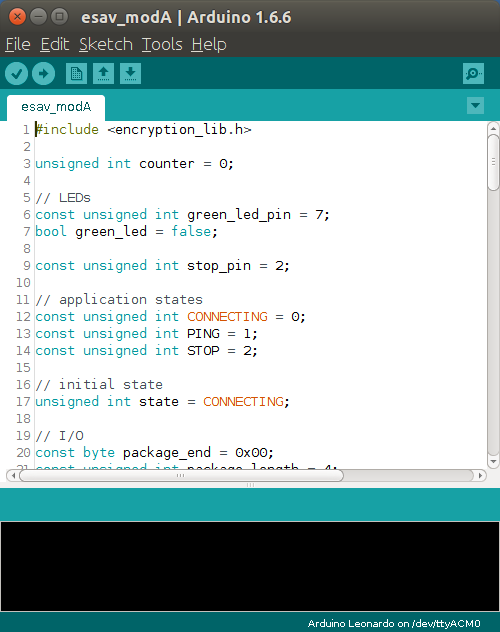
\includegraphics[scale=0.5]{pics/arduino_ide.png}
	\caption{\label{fig:arduino_ide}Interfejs programu Arduino IDE używany do programowania na platformę Arduino (zdjęcie: Piotr Banaszkiewicz).}
\end{figure}

\subsection{Kabel do programowania Arduino}
\label{subsec:kabel_do_programowania_arduino}

Platforma Arduino Pro, w przeciwieństwie do innych większych mikrokontrolerów Arduino, nie zawiera programatora na USB. Programowanie Arduino Pro odbywa się poprzez port szeregowy (6 pinów usytuowanych równolegle do płytki PCB, widocznych po lewej stronie na zdjęciu \ref{fig:arduino_pro}).

\begin{figure}[h]
	\centering
	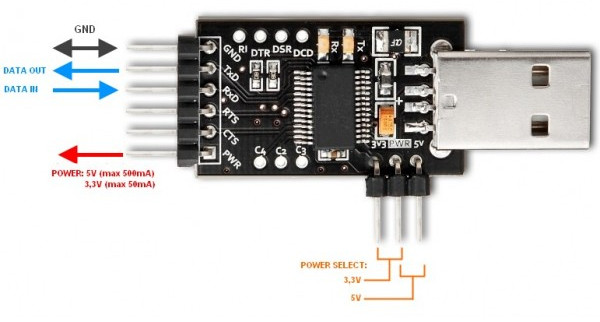
\includegraphics[scale=0.5]{pics/konwerter-usb-uart-ft232-33-5v.jpg}
	\caption{\label{fig:arduino_ide}Opis wyjść używanego konwertera USB-UART (zdjęcie: Botland \cite{KonwerterBotland}).}
\end{figure}

Niestety używany konwerter USB-UART posiada zgodne wyprowadzenia (zob. powyższe zdjęcie), ale w nieodpowiedniej kolejności, co zostało przedstawione w tabeli \ref{tab:piny}.

\begin{table}[h]
    \centering
    
    \begin{threeparttable}
        \caption{Złącza komunikacji szeregowej i zasilania platformy Arduino Pro oraz używanego konwertera USB-UART.}
        \label{tab:piny}
        
        \begin{tabular}{cc}
            \toprule
            Wyprowadzenie Arduino Pro & Wyprowadzenie konwertera USB-UART \\
            \midrule
            RST & GND \\
            TX & TXD \\
            RX & RXD \\
            5V & RTS \\
            GND & CTS \\
            GND & PWR \\
            \bottomrule
        \end{tabular}
        
    \end{threeparttable}
\end{table}

Podłączenia wymagane do prawidłowego zaprogramowania Arduino Pro:

\begin{itemize}
\item RST $\rightarrow$ RTS
\item TX $\rightarrow$ RXD
\item RX $\rightarrow$ TXD
\item 5V $\rightarrow$ PWR
\item GND $\rightarrow$ GND
\end{itemize}

W związku z tym konieczne stało się stworzenie kabla pozwalającego łatwo programować moduły systemu ESAV. Został on zbudowany na podstawie tzw. skrętki ethernetowej (zdjęcie \ref{fig:cable}).

\begin{figure}[h]
	\centering
	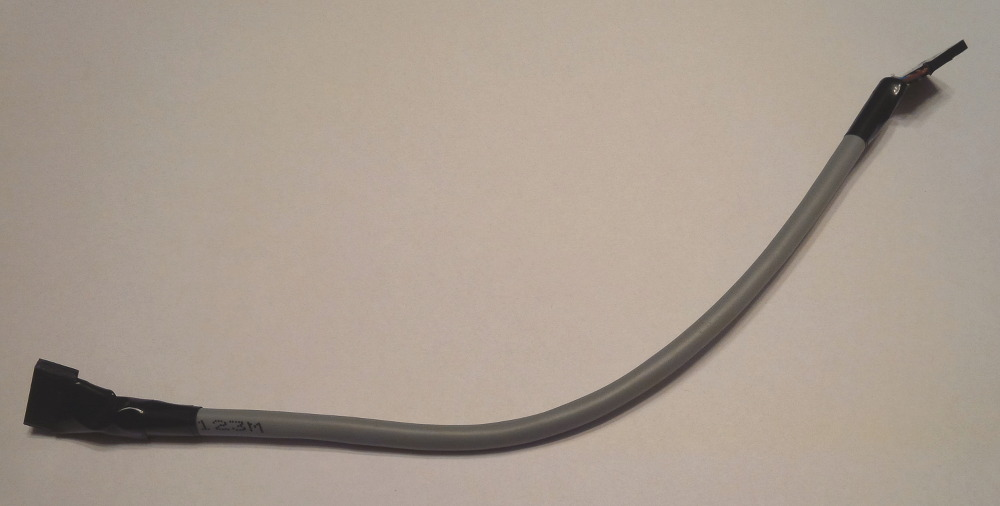
\includegraphics[scale=0.3]{pics/cable.jpg}
	\caption{\label{fig:cable}Zdjęcie kabla wykorzystywanego do programowania Arduino (zdjęcie: Piotr Banaszkiewicz).}
\end{figure}

Niestety tak krótki kabel ethernetowy (ok. $20\mathrm{cm}$) ma bardzo dużą sztywność i potrafi podnieść platformę Arduino, ponieważ ma ona niewielką masę.

%---------------------------------------------------------------------------

\section{Zakres zrealizowanych wymagań}
\label{sec:zrealizowane_wymagania}

W poniższej tabeli zestawiono założenia projektu wyszczególnione w rozdziale wraz z informacją o ich spełnieniu (bądź wytłumaczeniem dlaczego nie zostały spełnione) oraz odnośnikiem do rozdziału zawierającego bardziej szczegółowe informacje na temat danej funkcjonalności.

\begin{longtable}{p{.15\textwidth} p{.15\textwidth} p{.15\textwidth} p{.35\textwidth} p{.05\textwidth}}
\caption{Macierz śledzenia wymagań (ang. \textit{requirements traceability matrix} \cite{Hug10}).} \label{tab:spelnione_wymagania} \\

\toprule
Numer wymagania & Wymagane? & Spełnione? & Jak? & Ref. \\
\midrule

1.2.1 & Tak & Tak & Przekaźnik typu \textit{Normally Open}. & \ref{subsec:odlaczanie_zalaczanie_silnika} \\ \hline
1.2.2 & Tak & Tak & Oprogramowanie modułów A~i~B. & \ref{subsec:schematy_cykli_dzialan} \\ \hline
1.2.3 & Tak & Tak & Przekaźnik typu \textit{Normally Open} oraz oprogramowanie modułu B. & \ref{subsec:maszyna_stanow} \\ \hline
1.2.4 & Tak & Tak & Oprogramowanie modułu B. & \ref{subsec:maszyna_stanow} \\ \hline
1.2.5 & Tak & Tak & Oprogramowanie modułu B. & \ref{subsec:maszyna_stanow} \\ \hline
1.2.6 & Tak & Tak & Oprogramowanie modułów A i B. & \ref{subsec:maszyna_stanow} \\ \hline
1.2.7 & Tak & Tak & Podpięcie przycisku ,,RESET'' do pinu RESET modułu B. & \ref{subsec:panel_operatorski} \\ \hline
1.2.8 & Tak & Tak & Przekaźnik typu \textit{Normally Open}. & \ref{subsec:odlaczanie_zalaczanie_silnika} \\ \hline
1.2.9 & Nie & Nie & Zakupione powerbanki umożliwiają ładowanie podczas używania ich, jednakże to w gestii użytkownika jest korzystanie z tej możliwości. & \ref{subsec:zasilanie} \\ \hline
1.3.1 & Tak & Tak & Powerbanki powinny teoretycznie zapewnić zasilanie przez około 50–100 godzin. & \ref{subsec:zasilanie} \\ \hline
1.3.2 & Tak & Tak & Prędkość przesyłania danych między modułami HC-12 wynosi 5000bps. & \ref{subsec:komunikacja} \\ \hline
1.3.3 & Tak & Tak & Przetestowano &  \\ \hline  %% podaj wartosc
1.3.4 & Tak & Tak & Przetestowano &  \\ \hline  %% podaj wartosc
1.4.1 & Tak & Tak & Moduł B odłącza zasilanie modułu, który bezpośrednio zasila silnik samochodu. & \ref{subsec:odlaczanie_zalaczanie_silnika} \\ \hline
1.4.2 & Nie & Nie & Zakupione powerbanki umożliwiają ładowanie podczas używania ich, jednakże to w gestii użytkownika jest korzystanie z tej możliwości. & \ref{subsec:zasilanie} \\ \hline
1.5.1 & Tak & Tak & Wejście sterowania przekaźnika jest zabezpieczone diodą gaszącą. & \ref{subsec:odlaczanie_zalaczanie_silnika} \\ \hline  %% uaktualnij!
1.5.2 & Tak & Tak & Komunikacja pomiędzy modułami polega na wymianie szyfrowanego licznika. & \ref{subsec:szyfrowanie_komunikacji} \\ \hline
1.6.1 & Nie & Nie & Poziom naładowania jest wyświetlany na obudowie powerbanku, więc nie ma konieczności dodatkowego monitorowania przez moduł B. & \ref{subsec:zasilanie} \\ \hline
1.6.2 & Tak & Tak & Spełnione dosłownie. & \ref{subsec:panel_operatorski} \\ \hline
1.6.3 & Tak & Tak & Spełnione dosłownie. & \ref{subsec:panel_operatorski} \\ \hline
1.6.4 & Tak & Tak & Spełnione dosłownie. & \ref{subsec:panel_operatorski} \\ \hline
1.6.5 & Nie & Nie & Poziom naładowania jest wyświetlany na obudowie powerbanku, więc nie ma konieczności dodatkowego monitorowania przez moduł B. & \ref{subsec:zasilanie} \\ \hline
1.6.6 & Tak & Tak & Spełnione dosłownie. & \ref{subsec:panel_operatorski} \\ \hline
1.6.7 & Tak & Tak & Spełnione dosłownie. & \ref{subsec:obudowy_montaz} \\ \hline
1.6.8 & Tak & Tak & Wysłanie pakietu danych jest rozumiane jako ,,PING''. & \ref{subsec:format_pakietow} \\ \hline
1.6.9 & Tak & Tak & Opisane w formacie pakietów. & \ref{subsec:format_pakietow} \\ \hline
1.6.10 & Nie & Nie & Niewymagane. &  \\ \hline

\bottomrule
\end{longtable}

%---------------------------------------------------------------------------

\section{Podsumowanie}
\label{sec:podsumowanie_specyfikacja_projektu}




\printbibliography

\end{document}
